\documentclass{rbfin}
\usepackage{amsmath}
\usepackage{amssymb} %mathbb
\usepackage{gensymb} % \degree
\usepackage{graphicx}
\usepackage{hyperref}

\begin{document}
\selectlanguage{brazil}
\shorttitle{Otimização Não Linear 2021} % appears on header every other page
\rbfe{}
\autor{Vinícius Claudino Ferraz, 2021}

\begin{center}
\Large

\textbf{Lista 4}

\normalsize

Matrícula $= 2019435823$
\end{center}

\large

\textbf{Questão 1}

\normalsize

\vspace{6mm}

\doublespacing

Ache a solução do problema a seguir utilizando um método gráfico.

Minimizar $f(x, y ) = x^2 + 2y^2 -2xy - 14x - 14y + 10$

sujeito a $g(x, y) = 4x^2 + y^2 - 25 \le 0$.

Minimizei $\varphi(x,y) = f(x,y) + 10^5 \cdot \max[0,g(x,y)]^2$ e verifiquei que o mínimo ocorre em $X^* = (2, 3)$ com $f(X^*) = -50$. 

Abaixo as curvas de nível de $\varphi$:

\begin{center}
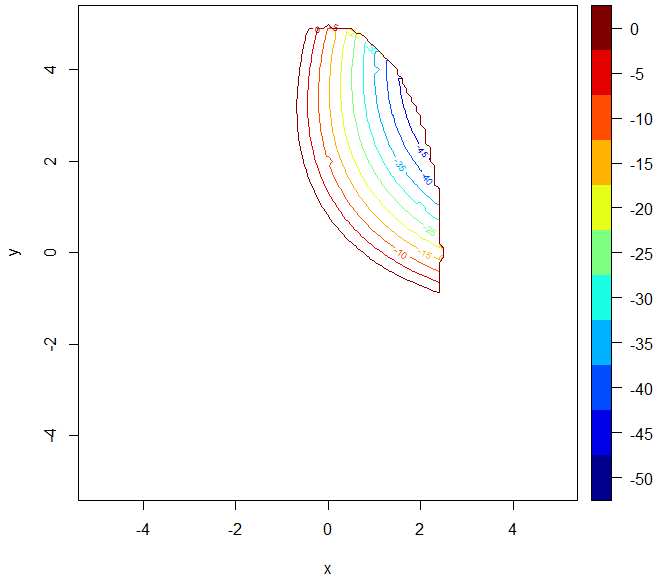
\includegraphics[scale=0.75]{H}
\end{center}

\newpage

Vemos abaixo o encontro da elipse $g(x,y) = 0$ com as curvas de nível de $f(x,y)$. O mínimo ocorre no tangenciamento.

\begin{center}
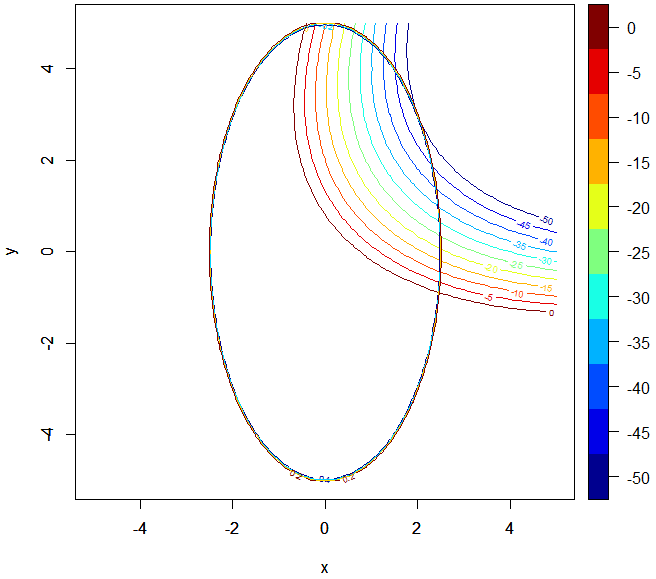
\includegraphics[scale=0.75]{FG}
\end{center}

Abaixo os fontes em R:

\singlespacing

\begin{verbatim}
library('plot3D')

dev.off()
Mx1 <- -5
Mx2 <- 5
My1 <- -5
My2 <- 5
delta <- 0.1
x <- seq(Mx1, Mx2, delta)
y <- seq(My1, My2, delta)
F <- matrix(0,nrow=length(x),ncol=length(y))
G <- matrix(0,nrow=length(x),ncol=length(y))
H <- matrix(0,nrow=length(x),ncol=length(y))
u <- 1e5
for (i in 1:length(x))
  for (j in 1:length(y)) {
     F[i,j]<- x[i]^2 + 2*y[j]^2 -2*x[i]*y[j] - 14*x[i] - 14*y[j] + 10
     G[i,j]<- 4*x[i]^2 + y[j]^2 - 25
     H[i,j] <- F[i,j] + u * max(0,G[i,j])^2
  }

min(H)
for (i in 1:length(x))
  for (j in 1:length(y))
    if (H[i,j] == min(H)) {
       print(x[i])
       print(y[j])
    }

contour2D(F,x,y,colkey = NULL,zlim=c(-50,0)) 
par(new=T)
contour2D(G,x,y,colkey = NULL,zlim=0) 

contour2D(H,x,y,colkey = NULL,zlim=c(-50,0)) 
\end{verbatim}

\vspace{6mm}

\large

\textbf{Questão 2}

\normalsize

\vspace{6mm}

\doublespacing

Ache a solução do problema a seguir utilizando o método da Penalidade Exterior
em conjunto com um método analítico de otimização irrestrita. Considere $u\to \infty$
analiticamente.

Minimizar $f(x,y) = (2x-y)^2+(y+1)^2$

sujeito a $h(x,y) = x+y - 10 = 0$.

Sistema equivalente: Minimizar $\varphi(x,y,u) = f(x,y) + u [h(x,y)]^2 = (2x-y)^2+(y+1)^2 + u (x+y - 10)^2$.

\begin{align*}
\cfrac{\partial \varphi}{\partial x} &= 4(2x-y) + 2u(x+y - 10) = 0 \Rightarrow y = \cfrac{10u - ux - 4x}{u - 2}\\
\cfrac{\partial \varphi}{\partial y} &= -2(2x-y) + 2(y+1) + 2u (x+y - 10) = 0\\
&\Rightarrow - 2x + \cfrac{10u - ux - 4x}{u - 2} + \cfrac{10u - ux - 4x}{u - 2}+1 + ux+ u\cdot \cfrac{10u - ux - 4x}{u - 2} - 10u = 0\\
&\Rightarrow - 2x(u - 2) + 10u - ux - 4x + 10u - ux - 4x + u - 2 + ux(u - 2) + 10u^2 - u^2x - 4ux - 10u(u - 2) = 0\\
&\Rightarrow x = \cfrac{41u - 2}{10u + 4} \therefore \lim_{u \to \infty} x = 4,1\\
y &= \cfrac{10u - 4,1 \cdot u - 16,4}{u - 2} \therefore \lim_{u \to \infty} y = 5,9
\end{align*}

Portanto, o mínimo ocorre em $X^* = (4,1;5,9)$ com $f(X^*) = 52,9$.

\singlespacing

\vspace{6mm}

\large

\textbf{Questão 3}

\normalsize

\vspace{6mm}

\doublespacing

Construa a função penalizada $\varphi$ utilizando o método da Penalidade Exterior e
resolva o problema a seguir.

Minimizar $f(x) = (x-1)^2$

sujeito a $g_1(x) = 2-x \le 0$ e $g_2(x) = x - 4 \le 0$.

Sistema equivalente: Minimizar $\varphi(x,u,v) = f(x) + u \max[0,g_1(x)]^2 + v \max[0,g_2(x)]^2$. 

Caso $1$: $2 \le x \le 4 \Rightarrow \varphi(x,u,v) = (x-1)^2$

$\cfrac{\partial \varphi}{\partial x} = 2(x - 1) = 0 \therefore x = 1 < 2$. Absurdo.

\newpage

Caso $2$: $x \le 2 \Rightarrow \varphi(x,u,v) = (x-1)^2 + u (x - 2)^2$

\begin{align*}
\cfrac{\partial \varphi}{\partial x} &= 2(x-1) + 2u (x - 2) = 0 \Rightarrow x = \cfrac{2u + 1}{u + 1} \\
\therefore \lim_{u \to \infty} x &= 2\,\,;\,\,f(2) = 1
\end{align*}

Caso $3$: $x \ge 4 \Rightarrow \varphi(x,u,v) = (x-1)^2 + v (x-4)^2$

\begin{align*}
\cfrac{\partial \varphi}{\partial x} &= 2(x-1) + 2v (x - 4) = 0 \Rightarrow x = \cfrac{4v + 1}{v + 1} \\
\therefore \lim_{v \to \infty} x &= 4\,\,;\,\,f(4) = 9 > 1
\end{align*}

Portanto, o mínimo ocorre em $x^* = 2$ com $f(x^*) = 1$.

\singlespacing

\large

\textbf{Questão 4}

\normalsize

\vspace{6mm}

\doublespacing

Ache a solução do problema a seguir (conhecido como problema de Rosen-Suzuki)
utilizando a função fmincon do MatLab, ou função similar para otimização não
linear restrita de qualquer outra linguagem de programação. Utilize o ponto inicial
$X = (0, 0, 0, 0)^\top$:

Minimizar $f(X) = x_1^2 + x_2^2 + 2x_3^2 - x_4^2 - 5x_1 - 5x_2 - 21x_3 + 7x_4 + 100$

sujeito a $x_1^2 + x_2^2 + x_3^2 + x_1 - x_2 + x_3 - x_4 - 100 \le 0$;

$x_1^2 + 2x_2^2 + x_3^2 + 2x_4^2 - x_1 - x_4 - 10 \le 0$;

$2x_1^2 + x_2^2 + x_3^2 - 2x_1 - x_2 - x_4 - 5 \le 0$;

$-100 \le x_i \le 100, 1 \le i \le 4$.

O mínimo ocorre em $X^* = (0.8265341110; 0.6497276158; 2.0343783578; -1.3756362681)$ com $f(X^*) = 47.7576120498$.

Abaixo os fontes em MatLab:

\singlespacing

\begin{verbatim}
function [c,ceq] = nonLinearConstraint4D(x)
    c(1) = x(1)^2 + x(2)^2 + x(3)^2 + x(1) - x(2) + x(3) - x(4) - 100;
    c(2) = x(1)^2 + 2 * x(2)^2 + x(3)^2 + 2 * x(4)^2 - x(1) - x(4) - 10;
    c(3) = 2 * x(1)^2 + x(2)^2 + x(3)^2 - 2 * x(1) - x(2) - x(4) - 5;
    ceq = [];
end

fun = @(x)x(1)^2+x(2)^2+2*x(3)^2-x(4)^2-5*x(1)-5*x(2)-21*x(3)+7*x(4)+100;
lb = [-100,-100,-100,-100];
ub = [100,100,100,100];
A = [];
b = [];
Aeq = [];
beq = [];
x0 = [0,0,0,0];
nonlcon = @nonLinearConstraint4D;
x = fmincon(fun,x0,A,b,Aeq,beq,lb,ub,nonlcon);
fprintf('x1 = %.10f\n',x(1));
fprintf('x2 = %.10f\n',x(2));
fprintf('x3 = %.10f\n',x(3));
fprintf('x4 = %.10f\n',x(4));
fprintf('f(x) = %.10f\n',fun(x));
\end{verbatim}

\vspace{6mm}

\large

\textbf{Questão 5}

\normalsize

\vspace{6mm}

\doublespacing

Ache a solução do problema a seguir utilizando a função fmincon do MatLab, ou
função similar para otimização não linear restrita de qualquer outra linguagem de
programação. Utilize o ponto inicial $X = (0.5, 1.0)^\top$:

Minimizar $f(x_1, x_2) = x_1^2 + x_2^2 - 4x_1 - 6x_2$

sujeito a $x_1 + x_2 \le 2$;

$2x_1 + 3x_2 \le 12$;

$x_1 \ge 0$;

$x_2 \ge 0$.

O mínimo ocorre em $X^* = (0.5; 1.5)$ com $f(X^*) = -8.5$.

Abaixo os fontes em MatLab:

\singlespacing

\begin{verbatim}
fun = @(x)x(1)^2 + x(2)^2 - 4*x(1) - 6*x(2);
lb = [0,0];
ub = [];
A = [1,1;2,3];
b = [2;12];
Aeq = [];
beq = [];
x0 = [0.5,1.0];
x = fmincon(fun,x0,A,b,Aeq,beq,lb,ub);
fprintf('x1 = %.10f\n',x(1));
fprintf('x2 = %.10f\n',x(2));
fprintf('f(x) = %.10f\n',fun(x));
fun([0.5,1.5])
\end{verbatim}

\vspace{6mm}

Versão de 07/fevereiro/2022\footnote{Fora da caridade não há salvação.} por Vinicius Claudino Ferraz.

\end{document}
